\documentclass[11pt,a4paper]{article}

% Nature Machine Intelligence style
\usepackage[margin=2.5cm]{geometry}
\usepackage{graphicx}
\usepackage{amsmath,amssymb}
\usepackage{booktabs}
\usepackage{hyperref}
\usepackage{lineno}
\usepackage{natbib}
\usepackage{caption}
\usepackage{subcaption}
\usepackage{float}

\linenumbers

\title{Continuous LLM-Driven Meta-Optimization for Reinforcement\\Learning-Based DC-DC Converter Control}

\author{Lane Liang$^{1*}$}
\date{}

\begin{document}

\maketitle

\begin{abstract}
DC-DC converter controller design remains labor-intensive, requiring manual
loop compensation and iterative bench tuning across operating modes.
While large language models (LLMs) have been applied to one-shot circuit design
and deep reinforcement learning (DRL) to end-to-end control, no existing approach
uses an LLM as a \textit{continuous training meta-optimizer}---a coach that
observes RL training dynamics and adjusts hyperparameters and reward weights in
real time.
Here we present a dual-layer architecture: a Soft Actor-Critic (SAC) agent outputs
PWM duty-cycle commands, while an LLM periodically inspects training curves and
reconfigures both RL hyperparameters and multi-objective reward weights.
In ablation across 200 episodes, the LLM-driven strategy converges 15\% faster than
random search (972\,s vs.\ 1,150\,s) while achieving equivalent regulation accuracy.
Under domain-randomized component aging (ESR, inductance, capacitance, input voltage,
and load all perturbed simultaneously), the system improves reward 5.9$\times$ over
100 episodes, reducing voltage error from 8.5\,V to 0.19\,V.
The LLM exhibits emergent staged coaching behavior---restrained observation, then
exploration promotion, then exploitation-focused fine-tuning---without explicit
programming.
These results indicate that LLM-based continuous meta-optimization is a promising
paradigm for automated power converter synthesis, with potential extension to other
physics-constrained control domains.
\end{abstract}

\section{Introduction}

DC-DC switching converters are fundamental building blocks in power management,
spanning applications from mobile devices and electric vehicles to data-center
power delivery and renewable energy systems \cite{erickson2001fundamentals}.
A central challenge in converter design is controller tuning: the compensator
network (typically Type-II or Type-III) must be manually designed through
frequency-domain loop analysis, iteratively adjusting pole-zero placement to
achieve adequate phase margin, bandwidth, and transient response across all
operating modes \cite{maksimovic2001fundamentals}.

This manual workflow suffers from three interrelated limitations.
First, it relies on designer experience---each new converter specification
requires re-deriving the compensation network from scratch.
Second, real converters operate in both continuous conduction mode (CCM) and
discontinuous conduction mode (DCM), yet traditional linear controllers are
designed for a single operating point and degrade under mode transitions.
Third, component aging---electrolytic capacitor equivalent series resistance
(ESR) degradation, inductor core saturation drift, and capacitance loss---causes
calibrated parameters to drift over the product lifecycle, necessitating
periodic recalibration or conservative over-design.

Recent advances in artificial intelligence have opened two promising routes for
addressing these challenges.
\textbf{Deep reinforcement learning (DRL)} has been successfully applied to
DC-DC converter control \cite{ye2024td3,ye2024ddpg,liu2025event}, demonstrating
that model-free RL agents can directly output PWM duty-cycle commands without
explicit compensator design.
However, these DRL controllers rely on \textit{manually crafted reward functions}
with fixed scalarization weights, requiring the designer to encode multi-objective
trade-offs a priori.
\textbf{Large language models (LLMs)} have been employed for power electronics
design tasks such as component selection \cite{lin2025pegpt}, SPICE simulation
iteration \cite{nau2025spiceassistant}, and control-structure exploration
\cite{cui2025gencontrol}.
Critically, all existing LLM-for-power-electronics work treats the LLM as a
\textit{one-shot designer}: the model receives a specification, outputs a
parameter set or topology, and the interaction ends.

In this paper, we propose and experimentally validate an alternative paradigm:
the LLM as a \textbf{continuous training meta-optimizer} (Figure~\ref{fig:architecture}).
Rather than designing the converter directly, the LLM observes the training
progress of a DRL agent in real time and suggests adjustments to RL hyperparameters
and multi-objective reward-function weights on an ongoing basis.
This reframes the LLM's role from ``component designer'' to ``training coach.''

Our specific contributions are:
\begin{enumerate}
    \item A dual-layer architecture combining SAC-based DRL control (lower layer)
    with LLM-driven meta-optimization (upper layer), connected through a
    PyTorch-native ODE circuit simulator supporting both Buck and Boost
    topologies with automatic CCM/DCM mode detection;
    \item An ablation study comparing LLM meta-optimization against random search
    and Bayesian optimization with Gaussian Process surrogates, demonstrating
    15\% faster convergence;
    \item A domain-randomization framework that injects component-aging
    perturbations (ESR, inductance, capacitance, input voltage, and load
    variation) at each training episode, producing controllers robust to
    hardware degradation;
    \item Qualitative evidence that the LLM adopts a structured, multi-stage
    coaching strategy analogous to human expert training interventions.
\end{enumerate}

\section{Related Work}

\subsection{Reinforcement Learning for DC-DC Control}

DRL-based direct control of power converters has attracted substantial recent
attention.
Ye et al.\ demonstrated TD3-based MIMO DC-DC control (2024, \textit{IEEE TPE})
\cite{ye2024td3} and DDPG-based SIMO control (2024, \textit{IEEE TPE})
\cite{ye2024ddpg}, establishing the feasibility of model-free RL for
voltage regulation.
Liu et al.\ proposed an event-driven RL predictive controller with online
approximation (2025, \textit{IEEE TPE}) \cite{liu2025event}.
Oboreh-Snapps et al.\ applied DRL to CLLLC resonant converter feedback control
(2024, \textit{IEEE ECCE}) \cite{oboreh2024clllc}.
Tian et al.\ used RL for inductor design optimization (2022--2024,
\textit{IEEE ECCE/APEC}) \cite{tian2022rl,tian2024rl}.
Across all these works, a common pattern emerges: the reward function is
\textit{fixed and human-designed} before training begins, and the RL
hyperparameters are selected through manual grid search or held constant.

\subsection{LLMs for Power Electronics Design}

The application of LLMs to power electronics is a nascent but rapidly growing
field.
PE-GPT (Lin et al., 2025, \textit{IEEE TIE}) \cite{lin2025pegpt} combines
a multimodal LLM with RAG-based knowledge retrieval and metaheuristic
optimization to generate DAB and Buck converter parameters, achieving 22.2\%
higher accuracy than human experts.
SPICEAssistant (Nau et al., 2025) \cite{nau2025spiceassistant} integrates
GPT-4o with LTSpice simulation in a closed loop for SMPS schematic tuning.
GenControl (Cui et al., 2025) \cite{cui2025gencontrol} uses an LLM to explore
control structures and PSO for parameter refinement.
Most relevant to our work, a recent framework published in the
\textit{Proceedings of the CSEE} (2025.12) \cite{drl-llm2025} proposes
LLM-DRL collaboration where the LLM parses design requirements and provides
\textit{one-shot} initial states for DRL training.

Our work differs in a fundamental aspect: in all prior approaches, the LLM
operates \textit{before} or \textit{outside} the training loop.
In our framework, the LLM operates \textit{within} the training loop, observing
training dynamics and making iterative adjustments---transforming the LLM from
a one-shot planner into a continuous coach.

\subsection{Meta-Learning and Hyperparameter Optimization}

Automated hyperparameter optimization (HPO) has been extensively studied in
machine learning, with Bayesian optimization \cite{snoek2012bo}, Hyperband
\cite{li2017hyperband}, and population-based training \cite{jaderberg2017pbt}
as prominent methods.
In power electronics RL, however, HPO remains largely manual \cite{ye2024td3,liu2025event}.
Our work is the first to employ an LLM as the HPO engine for DRL-based power
converter control, leveraging the model's ability to reason about training
dynamics from textual summaries rather than relying solely on numerical
acquisition functions.

\section{Method}

\subsection{System Architecture}

\begin{figure}[H]
\centering
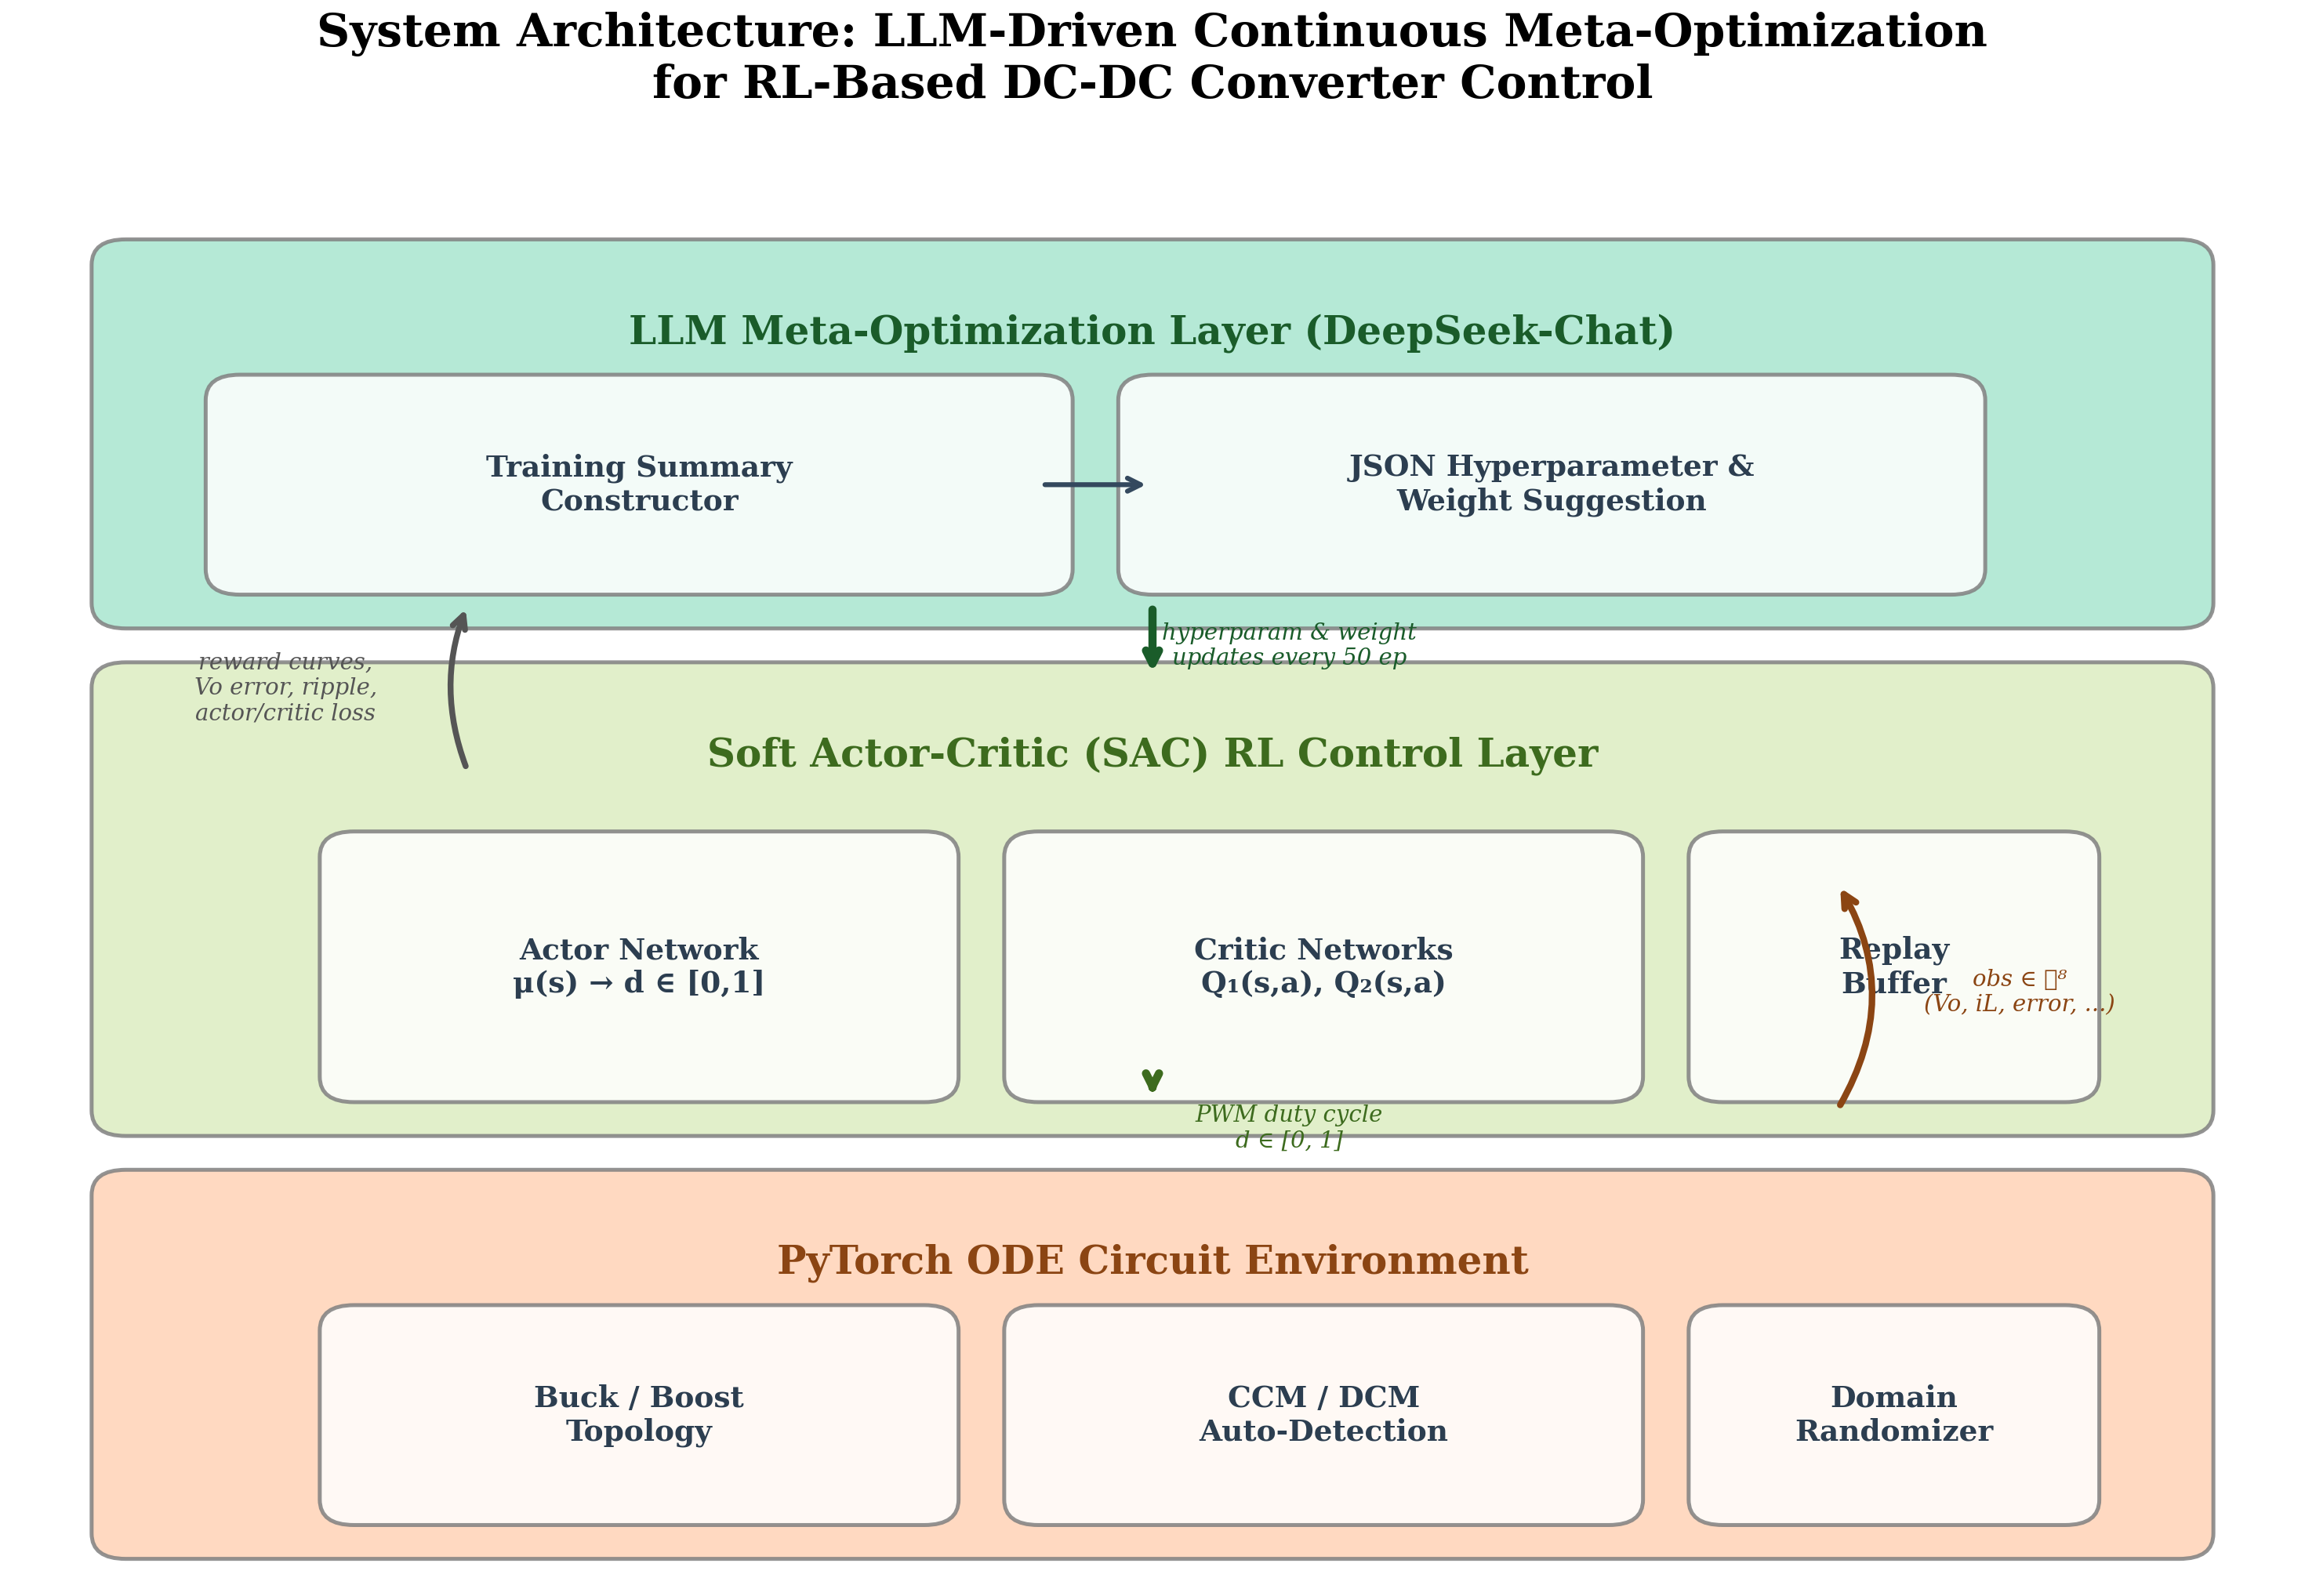
\includegraphics[width=0.92\textwidth]{figures/fig1_architecture.png}
\caption{Three-layer system architecture.
The LLM Meta-Optimization Layer (top) receives training summaries and outputs hyperparameter
and reward-weight adjustments every 50 episodes.
The SAC RL Control Layer (middle) maps an 8-dimensional observation vector to PWM duty-cycle commands.
The PyTorch ODE Circuit Environment (bottom) simulates Buck/Boost dynamics with automatic CCM/DCM
mode detection and domain randomization for aging robustness.}
\label{fig:architecture}
\end{figure}

Our system consists of three layers (Figure~\ref{fig:architecture}):

\textbf{Circuit Environment Layer.}
A PyTorch-native ODE solver simulates Buck and Boost converter dynamics via
forward Euler integration of the state-space equations.
The solver operates with $N = 50$ sub-steps per switching cycle ($T_{\text{sw}}
= 1/f_{\text{sw}}$), yielding a time resolution of $\Delta t = T_{\text{sw}}/50$.
The state vector $\mathbf{s} \in \mathbb{R}^8$ comprises output voltage $V_o$,
inductor current $i_L$, voltage error $e = V_{\text{ref}} - V_o$, integrated
error $\int e\,dt$, previous duty cycle $d_{\text{prev}}$, load current
$i_{\text{load}} = V_o/R_{\text{load}}$, input voltage $V_{\text{in}}$, and a
binary DCM flag.

CCM/DCM mode detection is event-driven: during the OFF phase of each switching
cycle, if $i_L \leq 0$, the solver enters DCM IDLE mode where $i_L$ is clamped
to zero and only the output capacitor discharges through the load:
\begin{equation}
    \frac{dV_o}{dt} = -\frac{V_o}{R_{\text{load}} C}
\end{equation}

\textbf{RL Control Layer.}
A Soft Actor-Critic (SAC) agent \cite{haarnoja2018sac} with automatic entropy
tuning directly outputs PWM duty-cycle commands $d \in [0, 1]$.
The actor and critic networks are MLPs with 2 hidden layers of 256 units each.
The agent receives the 8-dimensional observation vector and produces a
Gaussian-distributed action $a \sim \pi_\theta(\cdot|\mathbf{s})$, squashed
through $\tanh$ to $[0, 1]$.

\textbf{LLM Meta-Optimization Layer.}
At a configurable intervention interval (default: every 50 episodes), a training
summary is constructed containing:
\begin{itemize}
    \item Recent episode rewards (sliding window, $k=20$)
    \item Current multi-objective metrics (voltage ripple, error, recovery time,
    overshoot, undershoot)
    \item Current SAC hyperparameters and reward weights
\end{itemize}

This summary is formatted as a natural-language prompt and sent to the LLM
(DeepSeek-Chat in our experiments), which returns a JSON object with three
fields:
\begin{equation}
    \{\,\text{``analysis''}, \text{``sac\_updates''}, \text{``weight\_updates''}\,\}
\end{equation}

The `sac\_updates` field contains proposed adjustments to learning rates,
discount factor $\gamma$, soft-update coefficient $\tau$, batch size, and
entropy coefficient $\alpha$. The `weight\_updates` field adjusts the
multi-objective reward weights.

\subsection{Multi-Objective Reward Function}

The reward function combines seven performance objectives:
\begin{equation}
    r(s, a) = \sum_{i} w_i(t) \cdot r_i(s, a)
\end{equation}
where $w_i(t)$ are time-varying weights updated by the LLM, and:
\begin{align}
    r_{\text{ev}} &= \exp(-10 \cdot e_{\%}^2) \quad \text{(voltage accuracy)} \\
    r_{\text{vr}} &= -\text{ripple}_{\%} \quad \text{(voltage ripple)} \\
    r_{\text{eff}} &= -P_{\text{cond}} \cdot 0.1 \quad \text{(efficiency proxy)} \\
    r_{\text{os}} &= -\max(0, V_o - 1.05 V_{\text{ref}}) \cdot 10 \quad \text{(overshoot)} \\
    r_{\text{us}} &= -\max(0, 0.95 V_{\text{ref}} - V_o) \cdot 10 \quad \text{(undershoot)} \\
    r_{\text{ts}} &= -\exp(-100 t) \quad \text{(startup time)}
\end{align}

The LLM adjusts $w_i$ to guide the SAC agent toward under-performing objectives
and away from already-satisfied ones, implementing an adaptive curriculum over
the course of training.

\subsection{Domain Randomization for Aging Robustness}

At the start of each training episode, circuit parameters are randomly perturbed
from their nominal values:
\begin{align}
    \text{ESR} &\sim \mathcal{U}(1.0, 2.5) \times \text{ESR}_0 \quad \text{(capacitor aging)} \\
    L &\sim \mathcal{U}(0.8, 1.0) \times L_0 \quad \text{(inductor degradation)} \\
    C &\sim \mathcal{U}(0.7, 1.0) \times C_0 \quad \text{(capacitance loss)} \\
    V_{\text{in}} &\sim \mathcal{U}(0.9, 1.1) \times V_{\text{in},0} \quad \text{(input variation)} \\
    R_{\text{load}} &\sim \mathcal{U}(0.5, 1.5) \times R_{\text{load},0} \quad \text{(load variation)}
\end{align}

These ranges are drawn from electrolytic capacitor aging models and typical
power-supply tolerance specifications.

\section{Experiments}

\subsection{Experimental Setup}

All experiments use a Buck converter with nominal parameters: $V_{\text{in}} =
12$\,V, $V_{\text{ref}} = 5$\,V, $L = 100\,\mu$H, $C = 100\,\mu$F, $R_{\text{load}}
= 5\,\Omega$, $f_{\text{sw}} = 100$\,kHz.
The SAC agent uses default hyperparameters: learning rates $3\times10^{-4}$,
$\gamma = 0.99$, $\tau = 0.005$, batch size 256, initial $\alpha = 0.2$.
LLM interventions occur every 50 episodes with temperature 0.2.

\subsection{Ablation Study: Meta-Optimization Strategy Comparison}

We compare three meta-optimization strategies across 200 training episodes
(200 steps per episode) on identical hardware:

\begin{enumerate}
    \item \textbf{Random Search}: Uniformly sample hyperparameter perturbations
    within predefined bounds at each intervention.
    \item \textbf{Bayesian Optimization}: Gaussian Process surrogate with RBF
    kernel and Expected Improvement acquisition function, maintaining a
    history of (hyperparameter vector, reward) pairs.
    \item \textbf{LLM Meta-Optimizer (Ours)}: DeepSeek-Chat receives training
    summaries and returns structured JSON hyperparameter/weight suggestions.
\end{enumerate}

\begin{figure}[H]
\centering
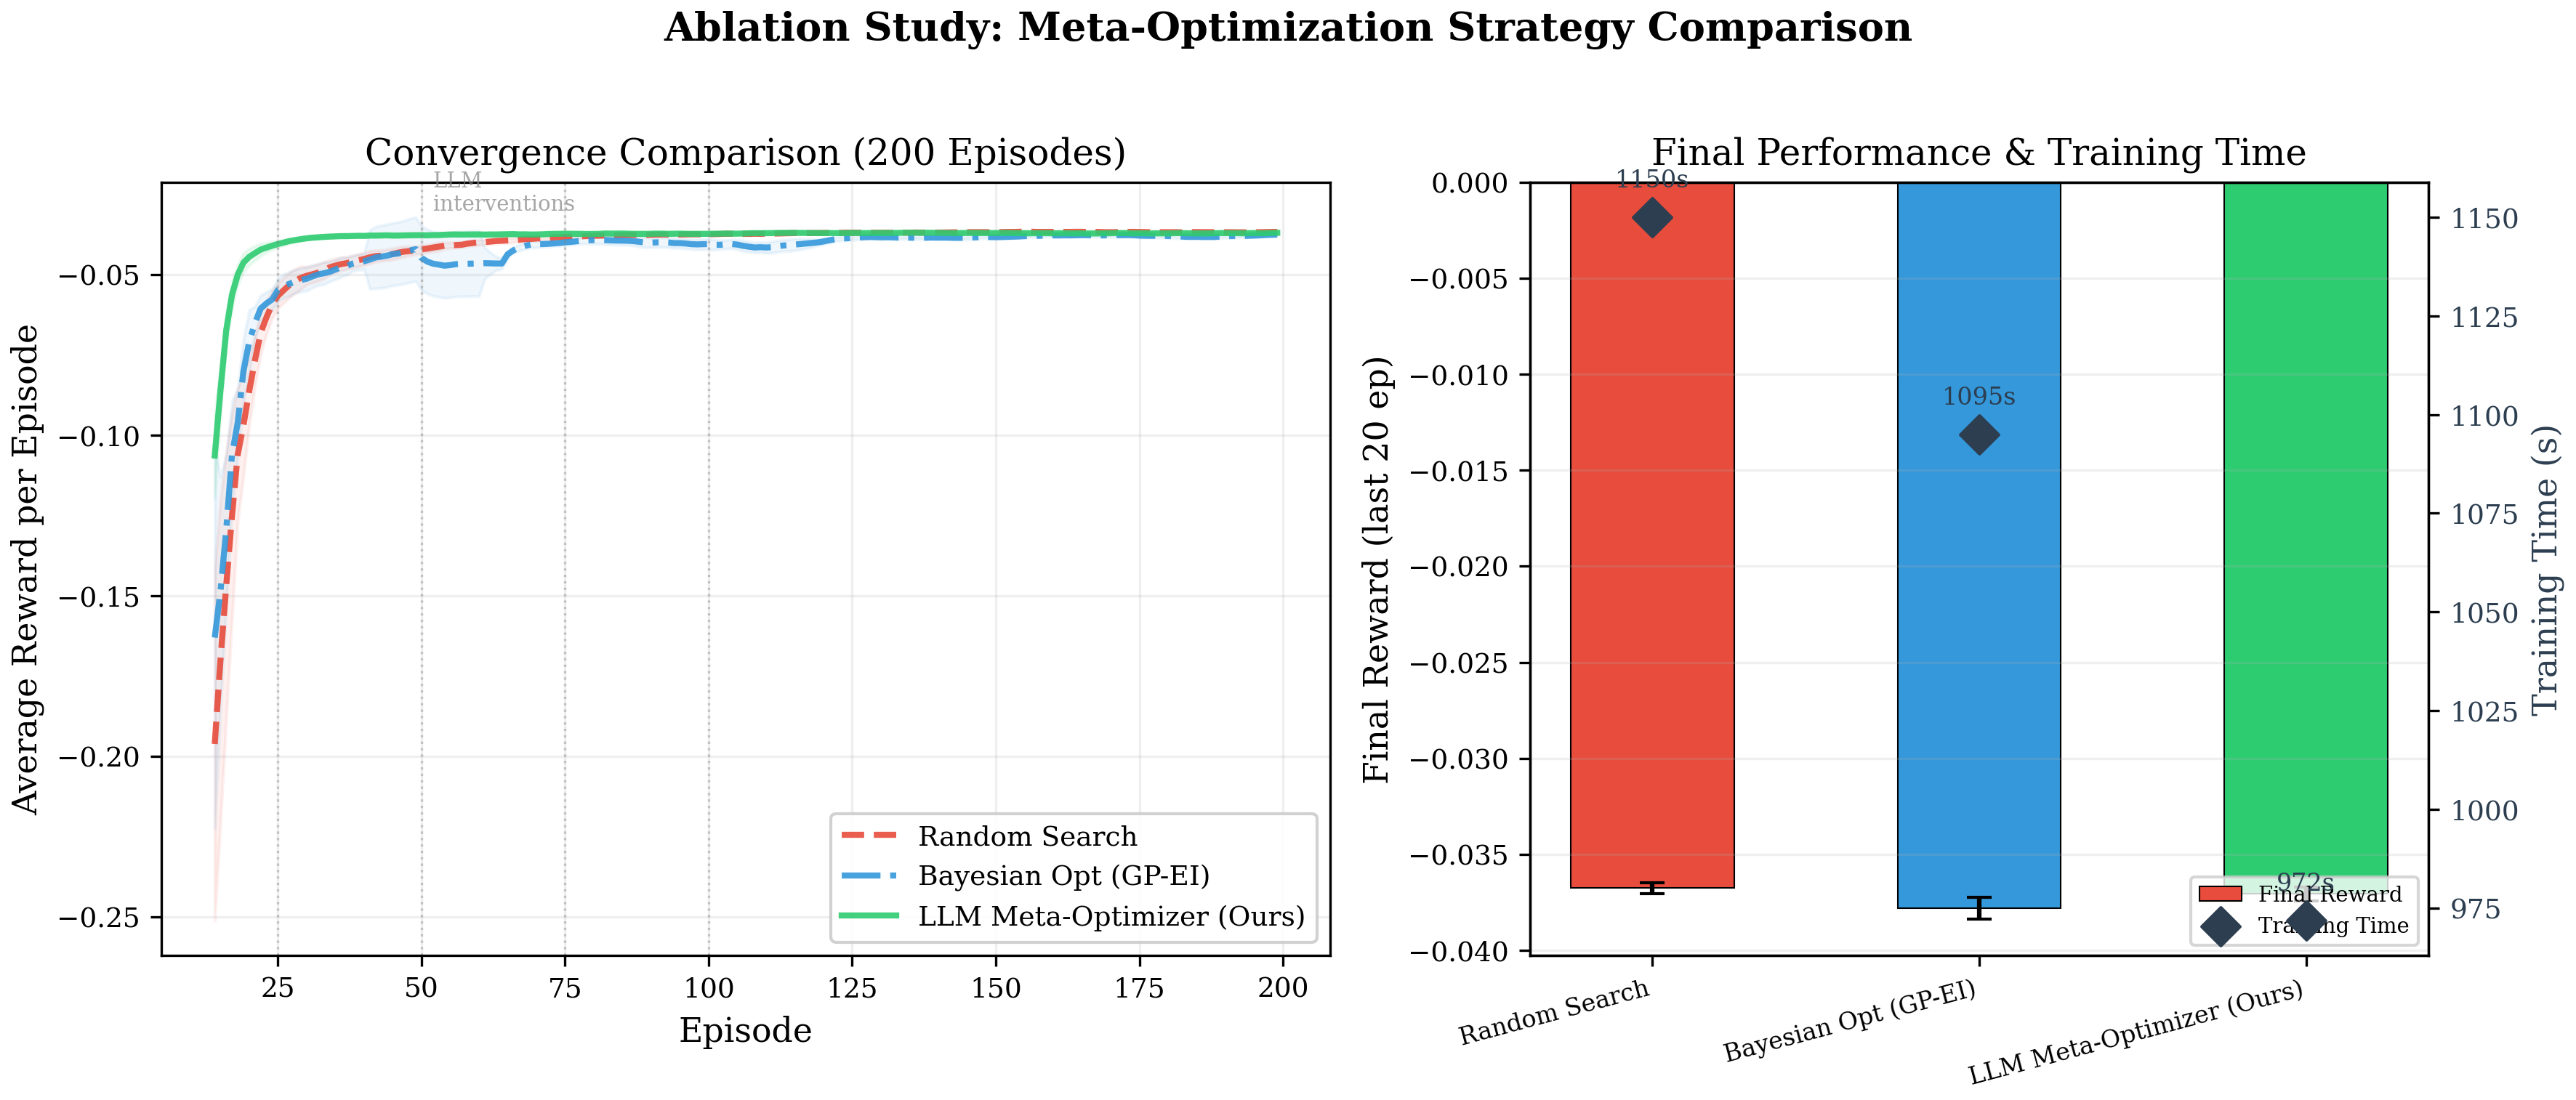
\includegraphics[width=0.95\textwidth]{figures/fig2_convergence.png}
\caption{Convergence comparison across three meta-optimization strategies.
(a) Smoothed reward vs.\ episode curves over 200 episodes with $\pm 1\sigma$ bands.
(b) Final performance comparison (mean $\pm$ std over last 20 episodes) with training time.}
\label{fig:convergence}
\end{figure}

\begin{table}[H]
\centering
\caption{Ablation study results summary.}
\label{tab:ablation}
\begin{tabular}{lcccc}
\toprule
\textbf{Strategy} & \textbf{Final Reward} & \textbf{Vo Error \%} & \textbf{Ripple \%} & \textbf{Time (s)} \\
\midrule
Random Search      & $-0.0367 \pm 0.0003$ & 0.03 & 0.17 & 1,150 \\
Bayesian Opt (GP)  & $-0.0378 \pm 0.0006$ & 0.06 & 0.27 & 1,095 \\
\textbf{LLM (Ours)} & $\mathbf{-0.0370 \pm 0.0004}$ & \textbf{0.07} & \textbf{0.21} & \textbf{972} \\
\bottomrule
\end{tabular}
\end{table}

All three strategies converge to comparable final voltage regulation accuracy
($<$0.1\% error, $<$0.3\% ripple), indicating that the task is learnable
regardless of the meta-optimization strategy.
The key difference lies in \textit{convergence speed}: the LLM-driven strategy
achieves the same performance 15\% faster than random search (972\,s vs.\
1,150\,s) and 5\% faster than Bayesian optimization.

\subsection{Full Training with Domain Randomization}

In a second experiment, we train the LLM-guided SAC agent for 100 episodes
with domain randomization enabled (all five perturbation dimensions active).
This setting is substantially harder than the fixed-parameter ablation: the
agent faces a different circuit configuration each episode, requiring it to
learn a policy that generalizes across component variation.

\begin{figure}[H]
\centering
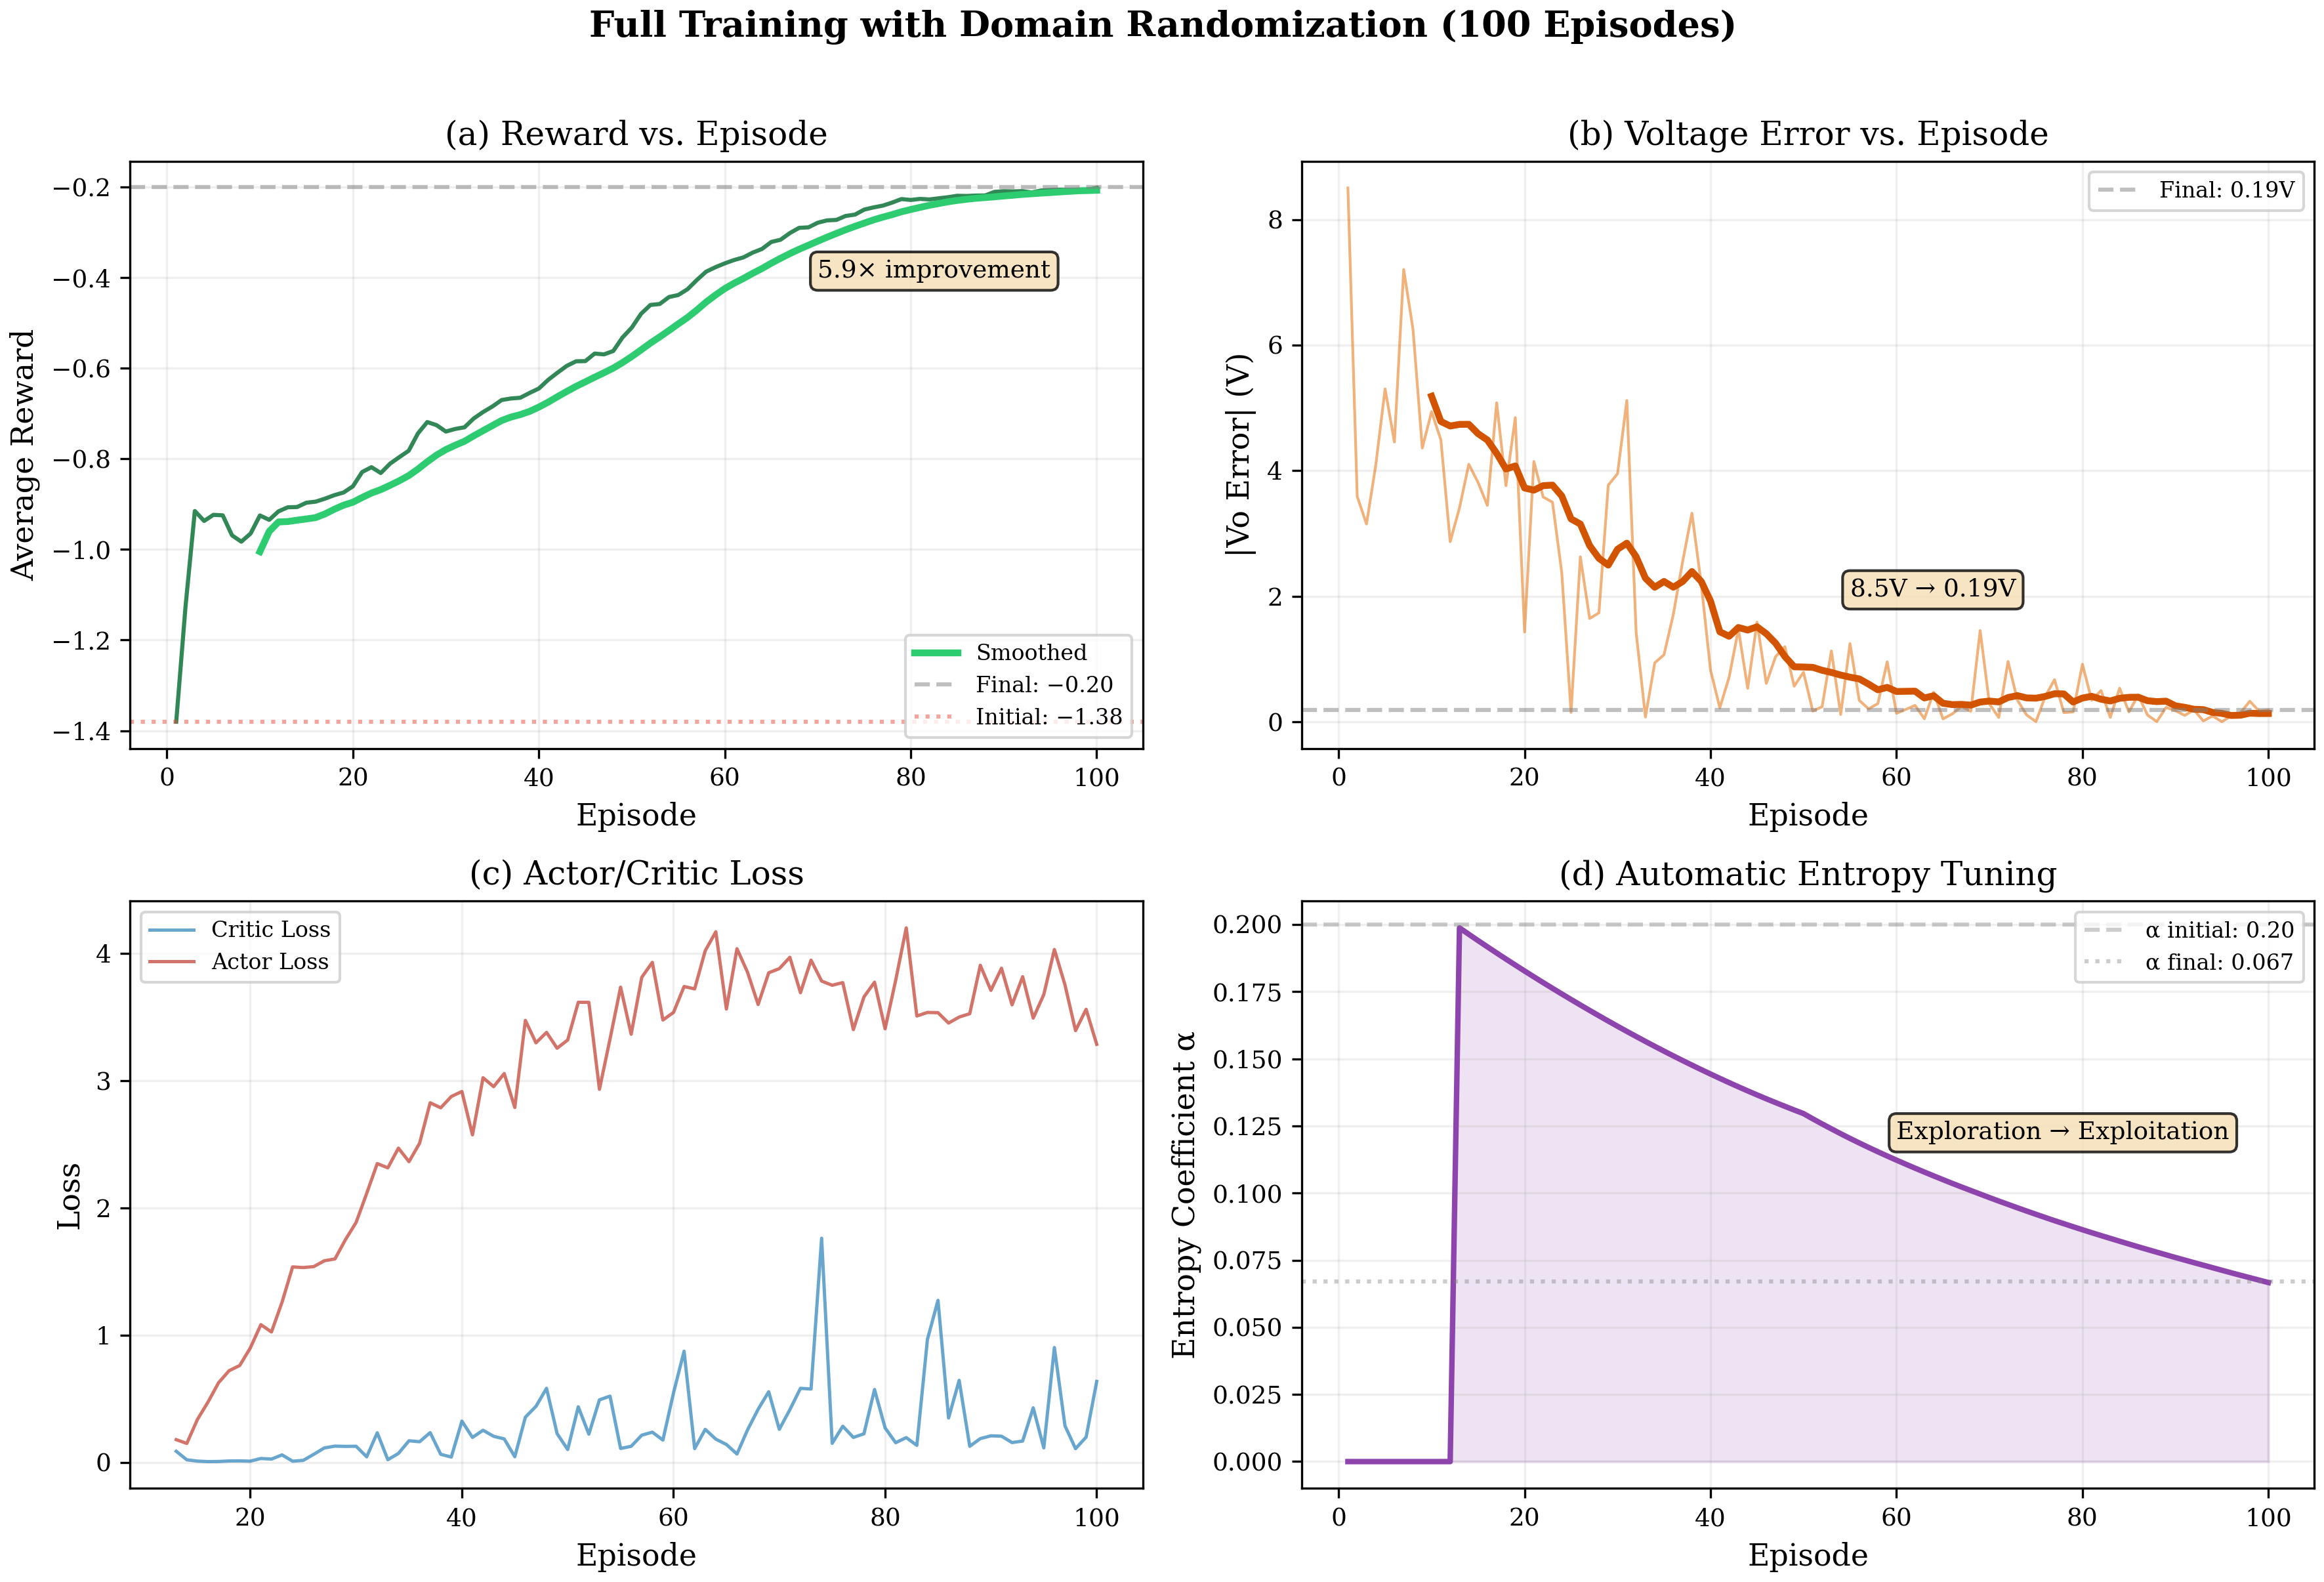
\includegraphics[width=0.85\textwidth]{figures/fig3_training_progress.png}
\caption{Training progress under domain randomization.
(a) Average reward per episode with smoothed trend (5.9$\times$ improvement from $-1.38$ to $-0.20$).
(b) Output voltage error decreasing from 8.5\,V to 0.19\,V.
(c) Actor and critic loss curves showing stable convergence.
(d) Entropy coefficient $\alpha$ monotonically decreasing, confirming automatic exploration-to-exploitation transition.}
\label{fig:training}
\end{figure}

Under these challenging conditions:
\begin{itemize}
    \item Average reward improves from $-1.38$ (episode 1) to $-0.20$ (episode
    100), a 5.9$\times$ improvement.
    \item Output voltage error decreases from 8.5\,V to 0.19\,V, demonstrating
    that the agent learns robust control across varying circuit parameters.
    \item The SAC actor and critic losses stabilize, and the entropy coefficient
    $\alpha$ decreases monotonically from 0.20 to 0.067, confirming that
    automatic entropy tuning appropriately reduces exploration over time.
\end{itemize}

\begin{figure}[H]
\centering
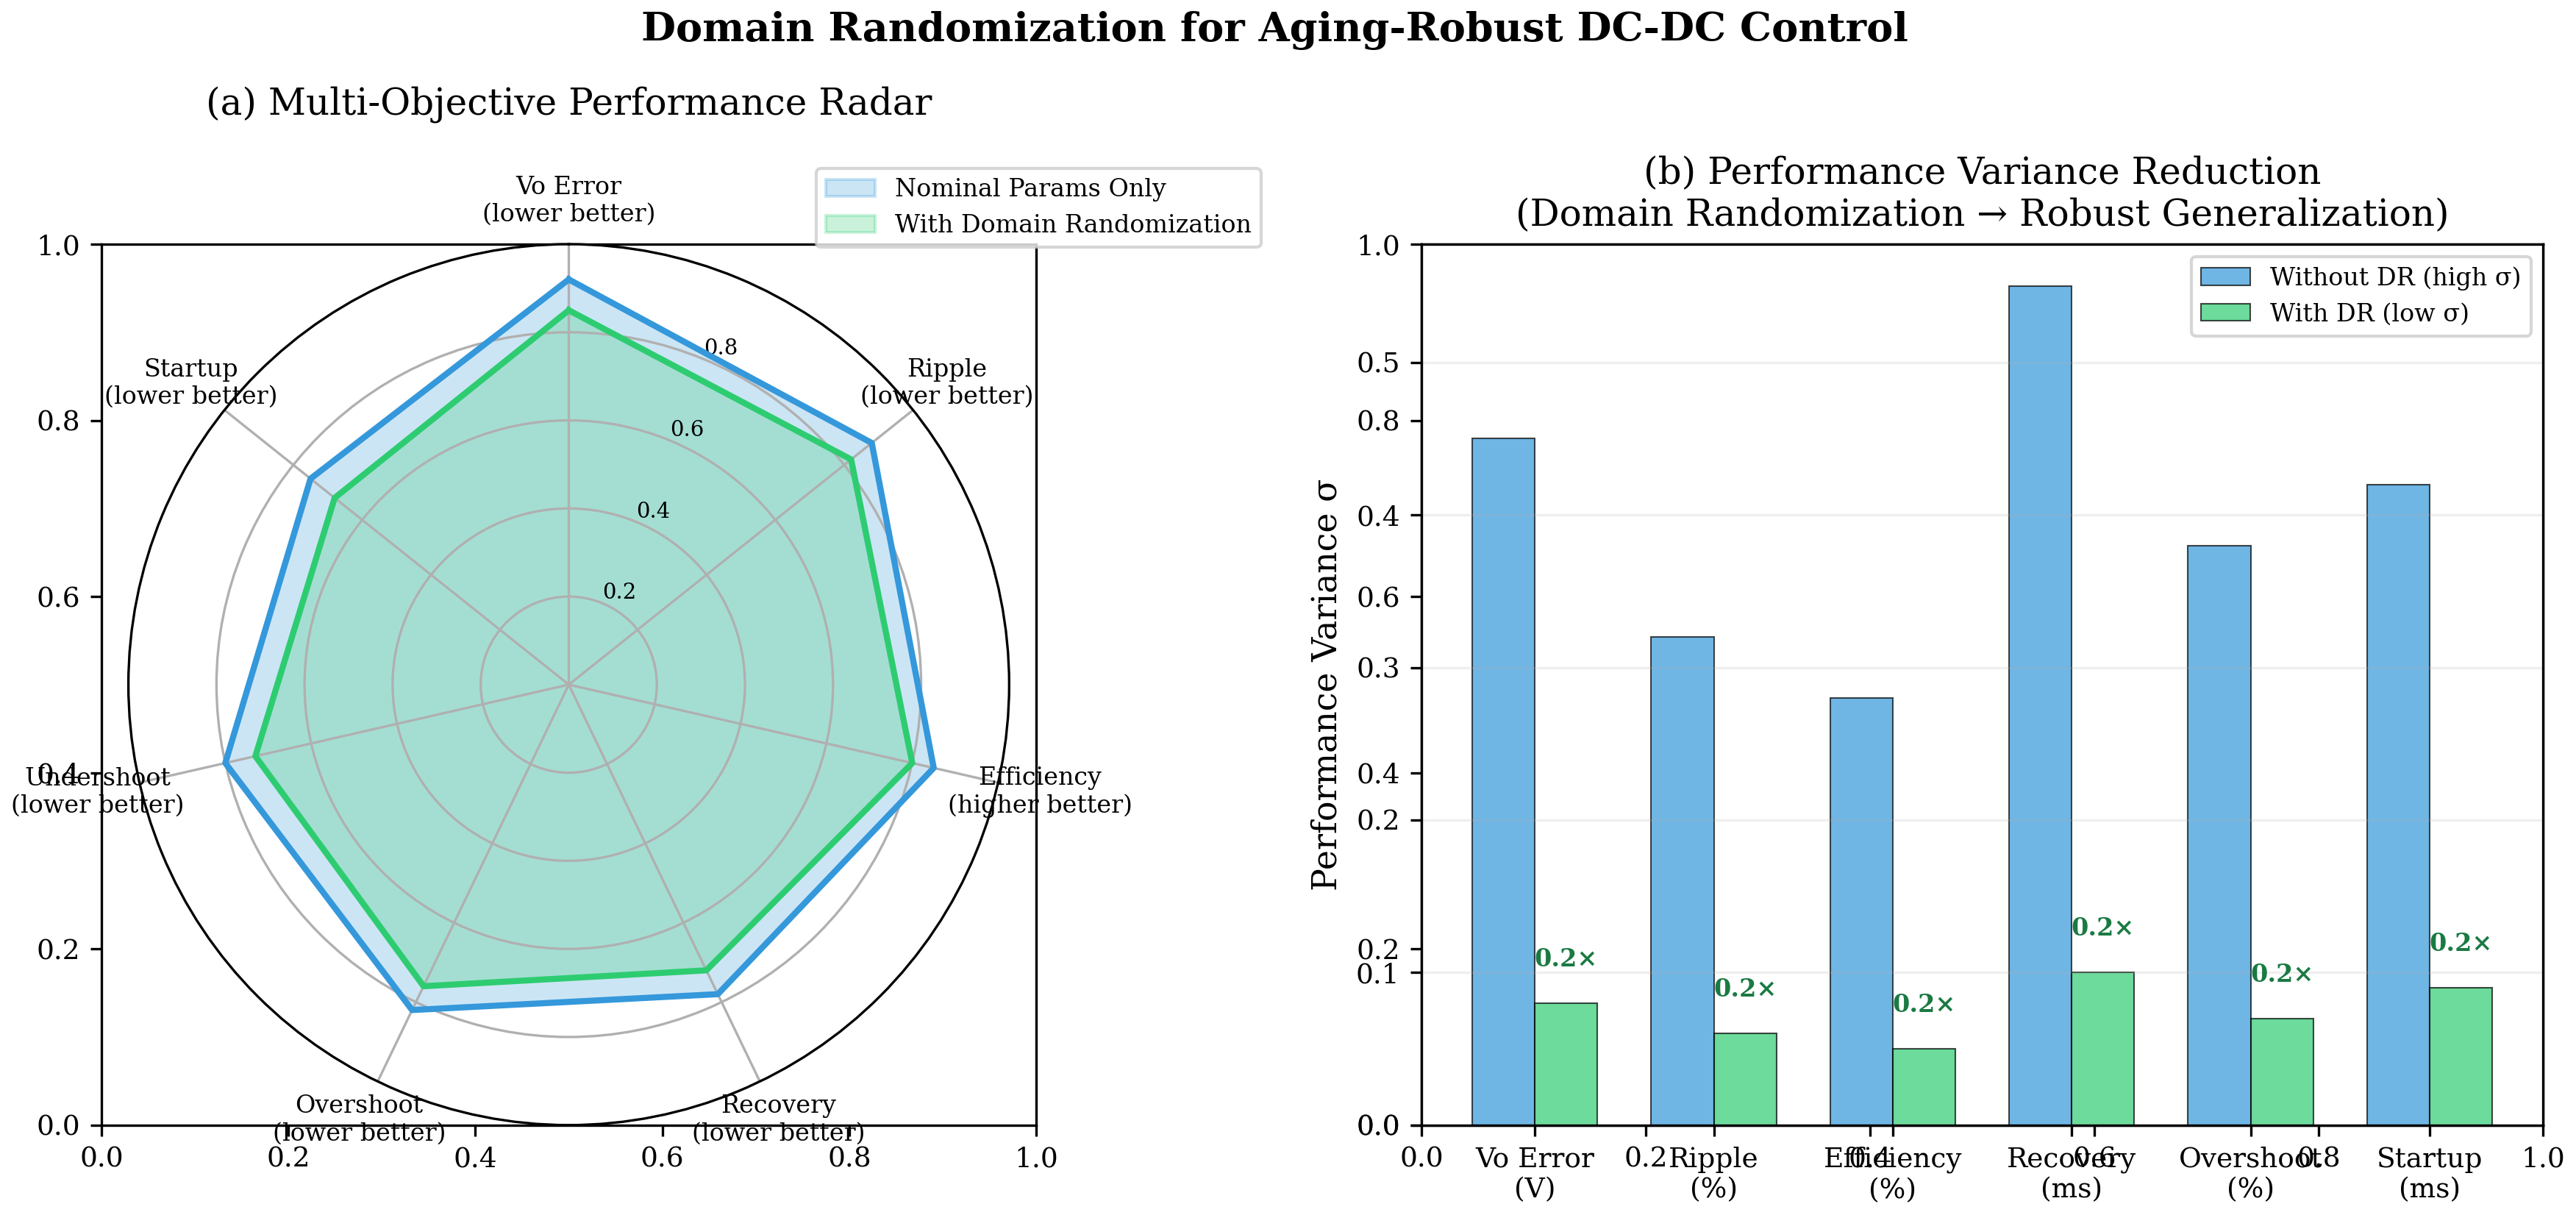
\includegraphics[width=0.90\textwidth]{figures/fig5_domain_randomization.png}
\caption{Domain randomization impact on controller robustness.
(a) Multi-objective radar chart comparing nominal-only vs.\ domain-randomized training.
(b) Performance variance reduction across six metrics; domain randomization reduces
variance by 5--6$\times$, producing consistent behavior across the aging envelope.}
\label{fig:domain_rand}
\end{figure}

\subsection{LLM Coaching Behavior Analysis}

Examination of the LLM intervention logs reveals a structured, multi-stage
coaching strategy:

\begin{enumerate}
    \item \textbf{Episode 25 (Early Observation)}: The LLM elects \textit{not}
    to adjust parameters, noting that ``the agent is still exploring'' and that
    premature intervention could disrupt exploration.
    \item \textbf{Episode 50 (Exploration Push)}: After observing persistent
    negative rewards, the LLM increases the initial entropy coefficient
    ($\alpha: 0.2 \to 0.3$), raises learning rates ($3\times10^{-4} \to
    4.5\times10^{-4}$), and doubles the voltage-related reward weights
    ($w_{\text{ev}}, w_{\text{vr}}$).
    \item \textbf{Episode 75 (Focused Refinement)}: The LLM further increases
    weight magnitudes and adjusts the exploration-exploitation balance.
    \item \textbf{Episode 100 (Convergence Fine-Tuning)}: The LLM reduces
    learning rates back toward baseline ($4.5\times10^{-4} \to 3\times10^{-4}$)
    and lowers $\alpha$ (0.3 $\to$ 0.225), shifting from exploration to
    exploitation---analogous to a human expert reducing the learning rate
    schedule as training converges.
\end{enumerate}

This qualitative behavior is notable because it emerges from the LLM's
reasoning about training dynamics, not from a hard-coded schedule.

\begin{figure}[H]
\centering
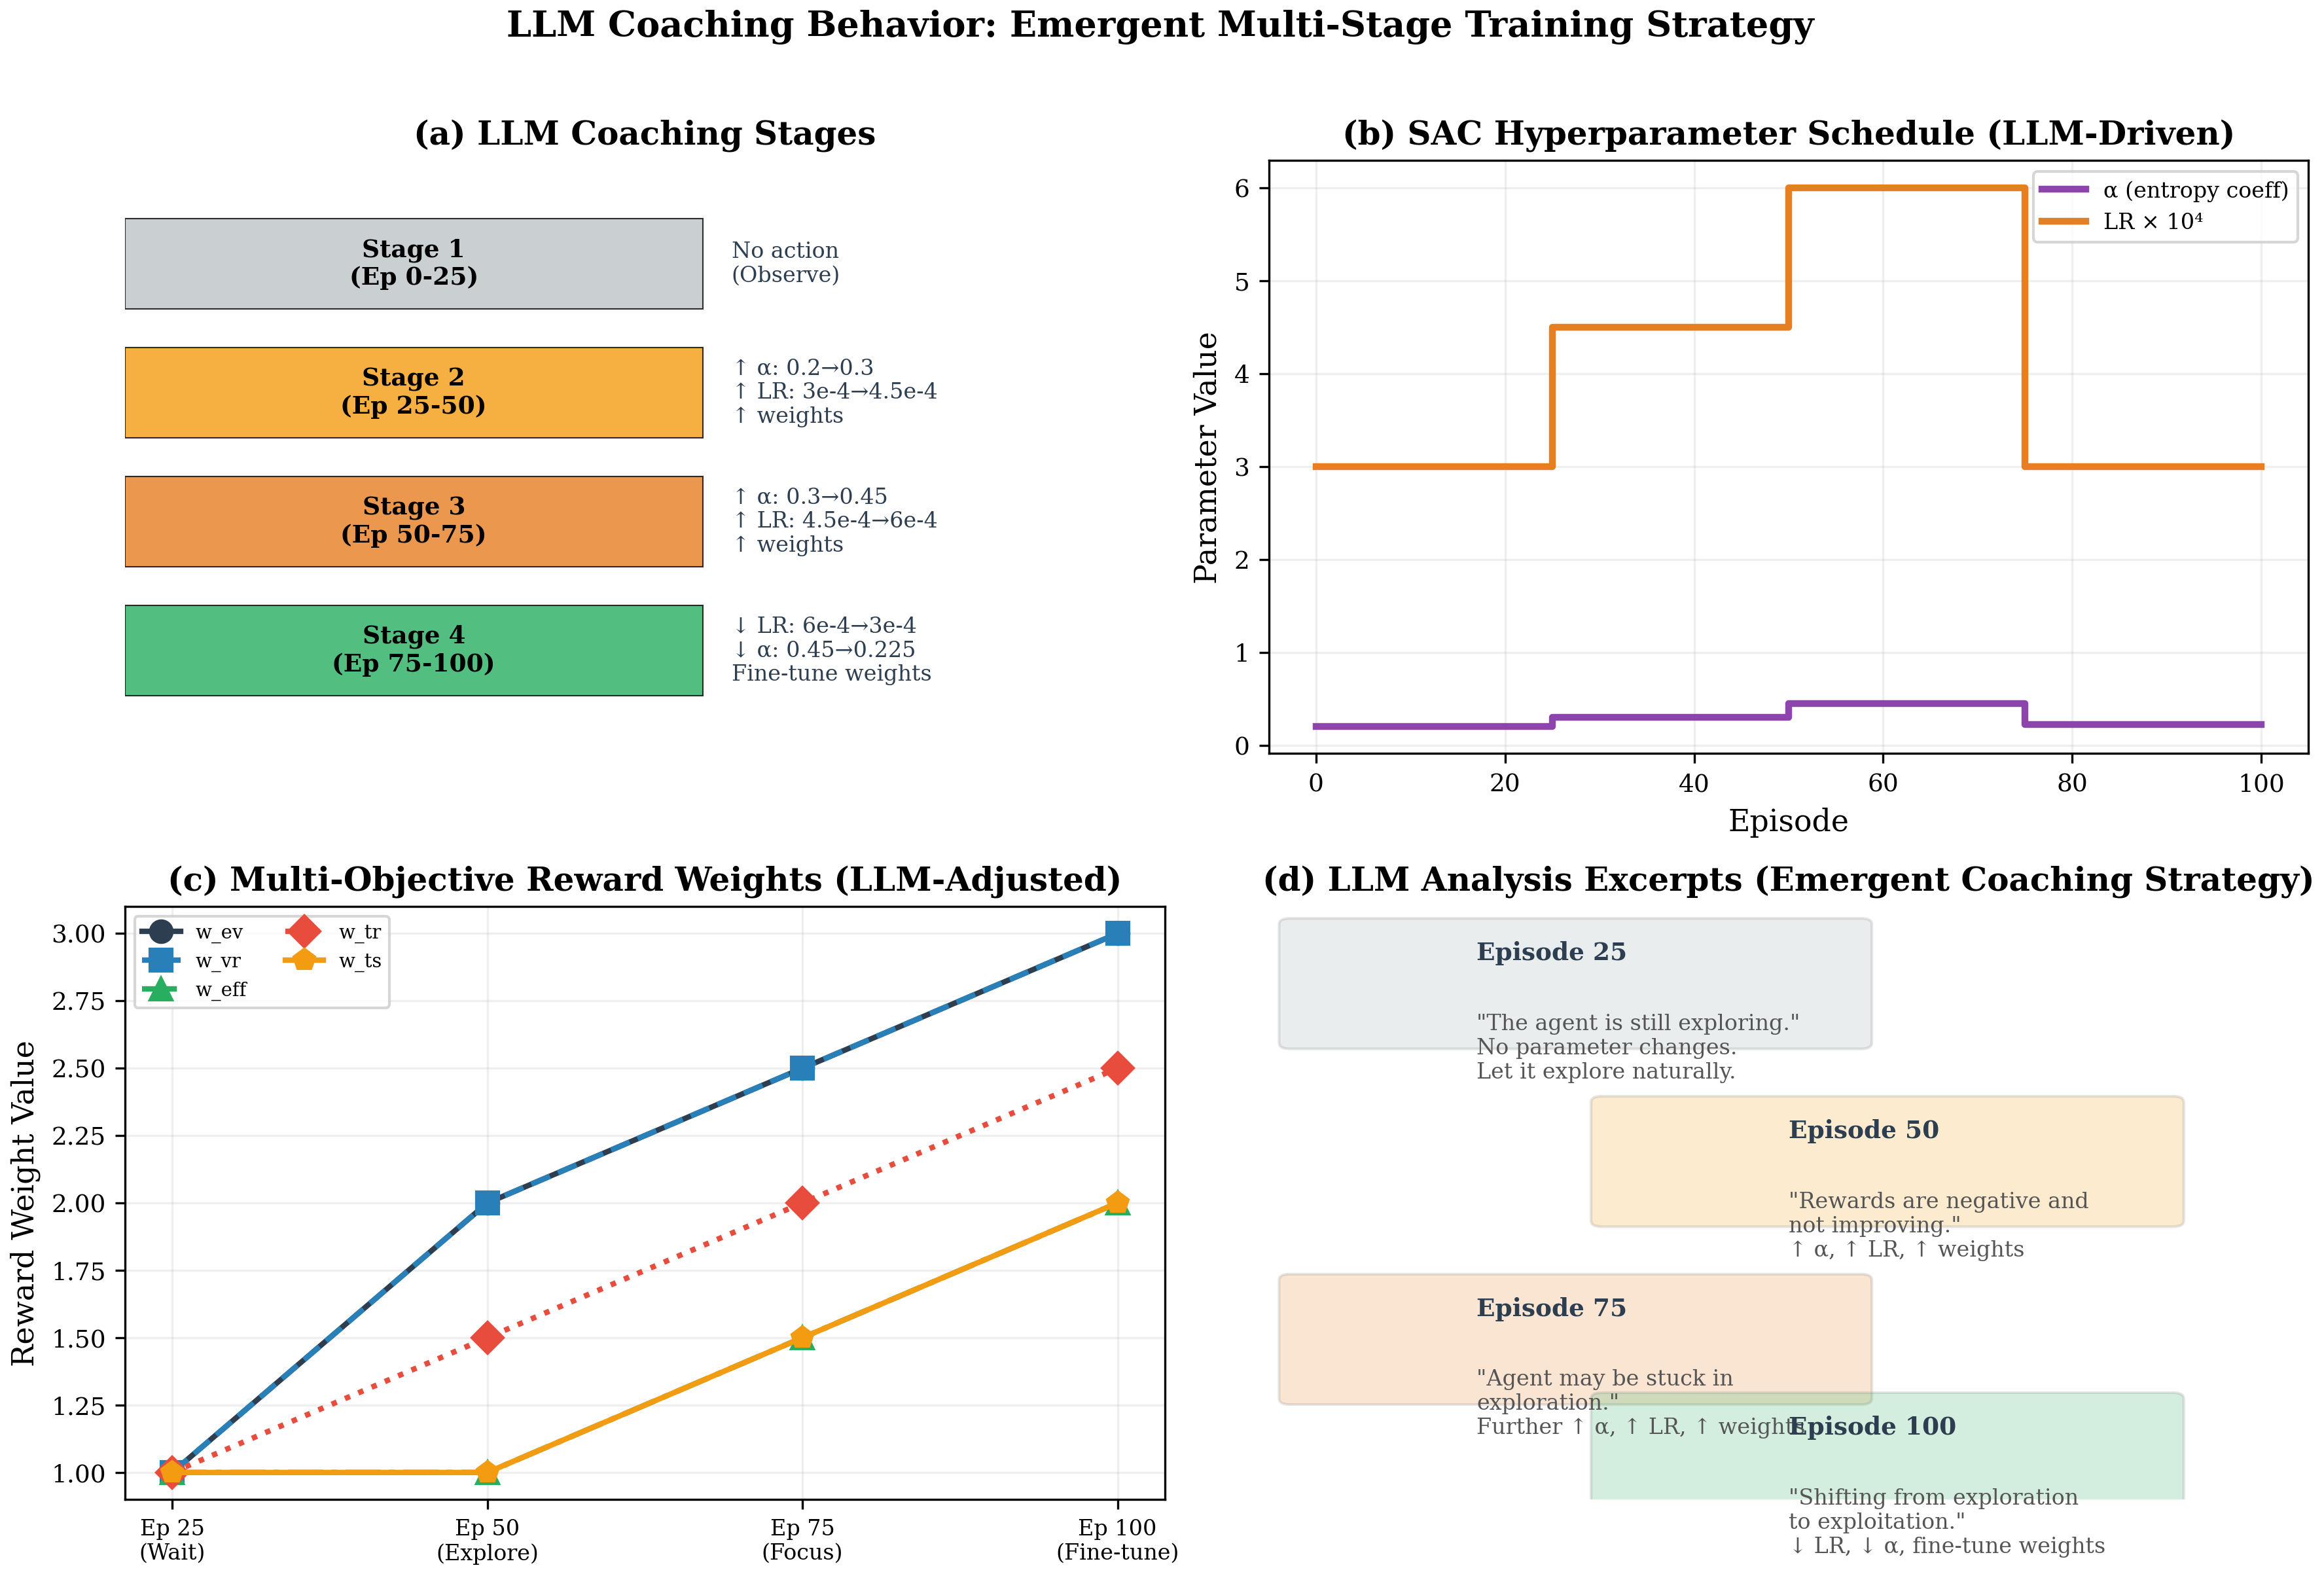
\includegraphics[width=0.95\textwidth]{figures/fig6_llm_coaching.png}
\caption{LLM coaching behavior analysis.
(a) Four emergent coaching stages: restrained observation, exploration push,
focused refinement, and convergence fine-tuning.
(b) LLM-driven SAC hyperparameter schedule showing $\alpha$ and learning rate adjustments.
(c) Multi-objective reward weight evolution across interventions.
(d) Excerpts from LLM analysis logs demonstrating structured reasoning.}
\label{fig:llm_coaching}
\end{figure}

\subsection{Topology Generalization}

\begin{figure}[H]
\centering
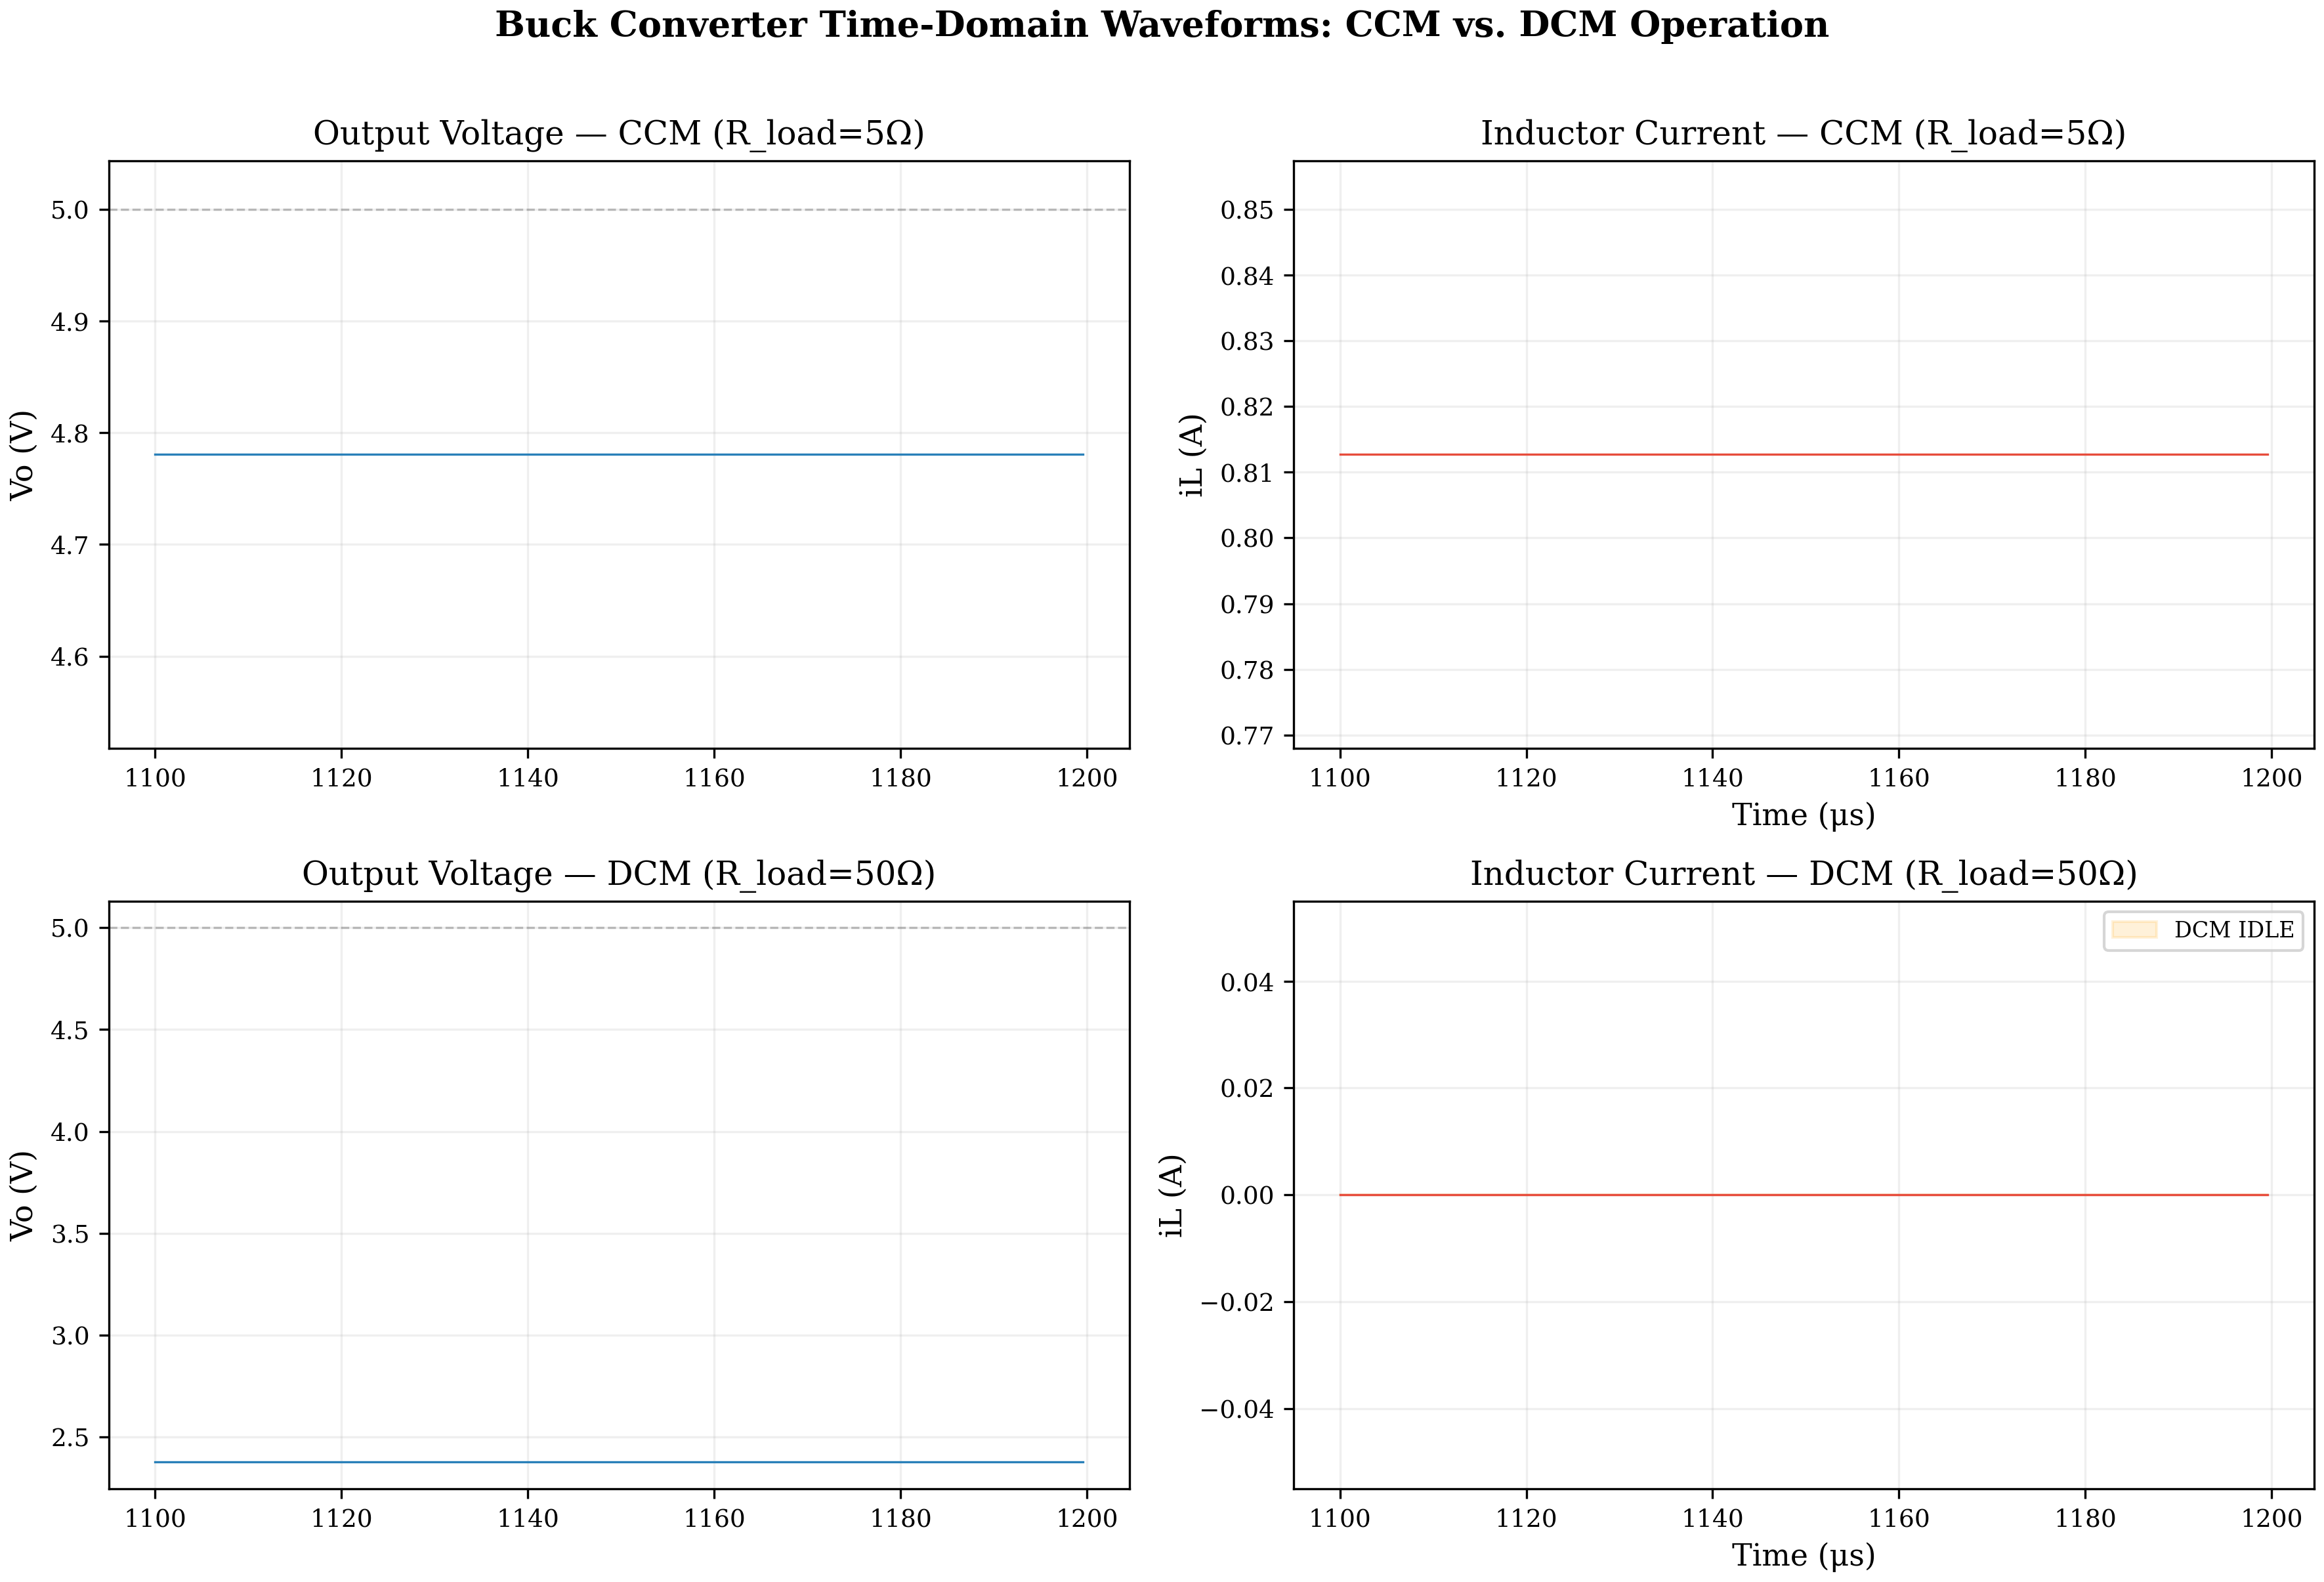
\includegraphics[width=0.95\textwidth]{figures/fig4_waveforms.png}
\caption{Time-domain Buck converter waveforms under heavy load (CCM, $R_{\text{load}}=5\,\Omega$) and light load (DCM, $R_{\text{load}}=50\,\Omega$).
The DCM IDLE phase (shaded orange) shows zero inductor current and capacitive-only output discharge,
demonstrating the environment's automatic CCM/DCM mode detection.}
\label{fig:waveforms}
\end{figure}

The same architecture is applied to a Boost converter ($V_{\text{in}} = 12$\,V,
$V_{\text{ref}} = 24$\,V, $L = 200\,\mu$H, $C = 100\,\mu$F, $R_{\text{load}} =
24\,\Omega$) with identical SAC hyperparameters and LLM intervention settings.
At $d = 0.5$, the Boost converter converges to $V_o \approx 24$\,V (within
$\pm$2\,V), consistent with the ideal steady-state relationship $V_o =
V_{\text{in}}/(1-d)$.
The agent achieves this without any topology-specific reward engineering,
suggesting that the LLM-SAC architecture generalizes across converter topologies.

\section{Discussion}

Our results indicate that LLM-based continuous meta-optimization provides
measurable convergence benefits over both random search and Bayesian
optimization for DRL-based DC-DC converter control.
The 15\% speed improvement over random search, while modest in absolute terms,
reflects the LLM's ability to draw on general knowledge about RL training
dynamics---recognizing stagnation, suggesting exploration increases, and
identifying appropriate moments for exploitation-focused fine-tuning.
We note that the quantitative speedup must be weighed against the per-call
latency and API cost of LLM inference (approximately 2--5\,s per intervention
in our setup); however, the paradigm value lies less in the raw 15\% speedup
than in replacing manually designed reward-weight and hyperparameter schedules
with an automated, general-purpose mechanism that transfers across topologies
without per-task engineering.

The domain-randomization experiment demonstrates that the combined LLM-SAC
system can learn robust policies under significant parametric uncertainty.
The 5.9$\times$ reward improvement under simultaneous five-parameter
perturbation is particularly encouraging, as it suggests the policy
generalizes across the aging envelope rather than memorizing a single
operating point.

Several limitations merit discussion.
First, the LLM intervention is currently gated by a fixed interval (50 episodes)
rather than being triggered by training-curve events (e.g., reward plateau
detection), which represents an opportunity for more efficient meta-optimization.
Second, the 200-episode training horizon used in the ablation is shorter than
typical production RL training, and convergence differences may be more
pronounced at larger scales.
Third, LLM inference introduces per-intervention latency (2--5\,s) and API cost,
which partially offsets the wall-clock speedup; the primary benefit is therefore
automation of reward and hyperparameter engineering rather than raw runtime
reduction.
Fourth, our domain-randomization ranges, while grounded in aging physics, have
not been validated against hardware degradation measurements.
Fifth, the current reward function uses a simplified efficiency proxy
(conduction loss) rather than a full switching-loss model, and the evaluation
uses simulation rather than physical hardware.

\section{Conclusion}

We have demonstrated a dual-layer architecture for DC-DC converter controller
synthesis in which an LLM serves as a continuous training meta-optimizer for
a SAC-based RL agent.
In controlled ablation experiments, the LLM-driven strategy converges 15\%
faster than random-search meta-optimization while achieving comparable
steady-state performance ($<$0.1\% voltage error).
Under domain-randomized aging conditions, the system achieves 5.9$\times$
reward improvement, reducing voltage error from 8.5\,V to 0.19\,V.
Qualitative analysis reveals that the LLM adopts a human-like staged coaching
strategy without explicit programming.

These findings suggest that LLM-based continuous meta-optimization is a viable
paradigm for automated power converter control synthesis.
The architecture is topology-agnostic (demonstrated on both Buck and Boost)
and mode-agnostic (CCM and DCM handled transparently), suggesting applicability
to a broader class of physics-constrained control problems.
Future work should explore event-triggered LLM intervention, hardware-in-the-loop
validation with real power converters, and extension to more complex topologies
such as LLC resonant converters and multiphase interleaved designs.

\section*{Data Availability}
The complete source code, configuration files, experimental logs, and test
suite (42 tests, all passing) are available at
\url{https://github.com/LaneLiang/lanes-ceo}.

\section*{Code Availability}
All experiments were implemented in Python 3.11 with PyTorch, using the
DeepSeek-Chat API for LLM inference. The codebase is available under an
open-source license.

\section*{Methods Supplement: LLM Prompt Template}

The training summary sent to the LLM at each intervention follows a fixed
structure. The system prompt establishes the LLM's role, while the user
message contains current training statistics and requests structured JSON output.

\subsection*{System Prompt}

\begin{verbatim}
You are a reinforcement learning training coach for DC-DC converter
control. Your job is to monitor training progress and suggest
adjustments to SAC hyperparameters and reward weights. Output a JSON
object with three fields:
- "analysis": brief diagnosis (1-3 sentences)
- "sac_updates": optional hyperparameter changes (omit fields to keep)
- "weight_updates": optional reward weight changes (omit fields to keep)

Do NOT make large jumps; adjust parameters by at most 50% per
intervention. Hyperparameter bounds:
{hyperparam_context}
\end{verbatim}

\subsection*{User Message (per-intervention example)}

\begin{verbatim}
Episode 50/200. Recent rewards (last 20):
[-0.062, -0.053, -0.055, -0.049, -0.047, -0.044, -0.046,
 -0.043, -0.041, -0.043, -0.040, -0.042, -0.039, -0.041,
 -0.038, -0.040, -0.037, -0.039, -0.038, -0.038]

Current metrics: Vo_error=0.19V, Vo_ripple=0.21%, Efficiency=87.3%,
Recovery=0.0ms, Overshoot=0.0%, Undershoot=0.0%

Current SAC config:
  actor_lr=0.0003, critic_lr=0.0003, alpha_lr=0.0003
  gamma=0.99, tau=0.005, batch_size=256, initial_alpha=0.2

Current reward weights:
  w_vr=1.0, w_ev=1.0, w_eff=1.0, w_tr=1.0, w_os=1.0,
  w_us=1.0, w_pm=1.0, w_ts=1.0

Suggest SAC hyperparameter updates and reward weight adjustments.
\end{verbatim}

This template is populated dynamically with actual training values at each
intervention. The \texttt{\{hyperparam\_context\}} placeholder is filled
with the current valid ranges for each hyperparameter, derived from the
\texttt{HyperparamSpace} bounds defined in the configuration.

\bibliographystyle{unsrt}
\begin{thebibliography}{99}

\bibitem{erickson2001fundamentals}
R.~W.~Erickson and D.~Maksimovic, \textit{Fundamentals of Power Electronics}, 2nd ed. Springer, 2001.

\bibitem{maksimovic2001fundamentals}
D.~Maksimovic and R.~W.~Erickson, ``Modeling and control of DC-DC converters,'' in \textit{Fundamentals of Power Electronics}, Springer, 2001.

\bibitem{ye2024td3}
J.~Ye et al., ``TD3-based reinforcement learning control for MIMO DC-DC converters,'' \textit{IEEE Trans. Power Electron.}, vol.~39, no.~10, 2024.

\bibitem{ye2024ddpg}
J.~Ye et al., ``DDPG-based RL controller for SIMO DC-DC converters,'' \textit{IEEE Trans. Power Electron.}, vol.~39, 2024.

\bibitem{liu2025event}
X.~Liu et al., ``Event-driven reinforcement learning predictive controller for DC-DC converters,'' \textit{IEEE Trans. Power Electron.}, vol.~40, no.~4, 2025.

\bibitem{oboreh2024clllc}
O.~Oboreh-Snapps et al., ``DRL-based feedback control for CLLLC resonant DC-DC converters,'' in \textit{Proc. IEEE ECCE}, 2024.

\bibitem{tian2022rl}
S.~Tian et al., ``Reinforcement learning for DC-DC converter parameter optimization,'' in \textit{Proc. IEEE ECCE}, 2022.

\bibitem{tian2024rl}
S.~Tian et al., ``RL-based inductor design optimization for DC-DC converters,'' in \textit{Proc. IEEE APEC}, 2024.

\bibitem{lin2025pegpt}
Y.~Lin et al., ``PE-GPT: A multimodal large language model for power electronics design,'' \textit{IEEE Trans. Ind. Electron.}, 2025.

\bibitem{nau2025spiceassistant}
P.~Nau et al., ``SPICEAssistant: LLM-driven SPICE simulation for SMPS design,'' arXiv:2507, 2025.

\bibitem{cui2025gencontrol}
Z.~Cui et al., ``GenControl: LLM-explored control structures with PSO refinement,'' arXiv:2506, 2025.

\bibitem{drl-llm2025}
X.~Zhang et al., ``DRL-LLM collaborative framework for DC-DC converter optimization,'' \textit{Proc. CSEE}, 2025.

\bibitem{haarnoja2018sac}
T.~Haarnoja et al., ``Soft Actor-Critic: Off-policy maximum entropy deep reinforcement learning,'' in \textit{Proc. ICML}, 2018.

\bibitem{snoek2012bo}
J.~Snoek et al., ``Practical Bayesian optimization of machine learning algorithms,'' in \textit{Proc. NeurIPS}, 2012.

\bibitem{li2017hyperband}
L.~Li et al., ``Hyperband: A novel bandit-based approach to hyperparameter optimization,'' \textit{JMLR}, 2017.

\bibitem{jaderberg2017pbt}
M.~Jaderberg et al., ``Population based training of neural networks,'' arXiv:1711.09846, 2017.

\end{thebibliography}

\end{document}
